\begin{fact} \label{iso-para}
	Considérons tous les parallélogrammes de périmètre fixé $p$. Parmi tous ces parallélogrammes, celui d'aire maximale est le carré de côté $c = \num{.25} p$.
\end{fact}


\begin{proof}
	Le calcul de l'aire d'un parallélogramme, voir le dessin ci-dessous, nous donne 
	$\area{ABCD} = \area{ABHH^{\,\prime}}$ et 
	$\perim{ABCD} \geq \perim{ABHH^{\,\prime}}$.	

	\begin{center}
		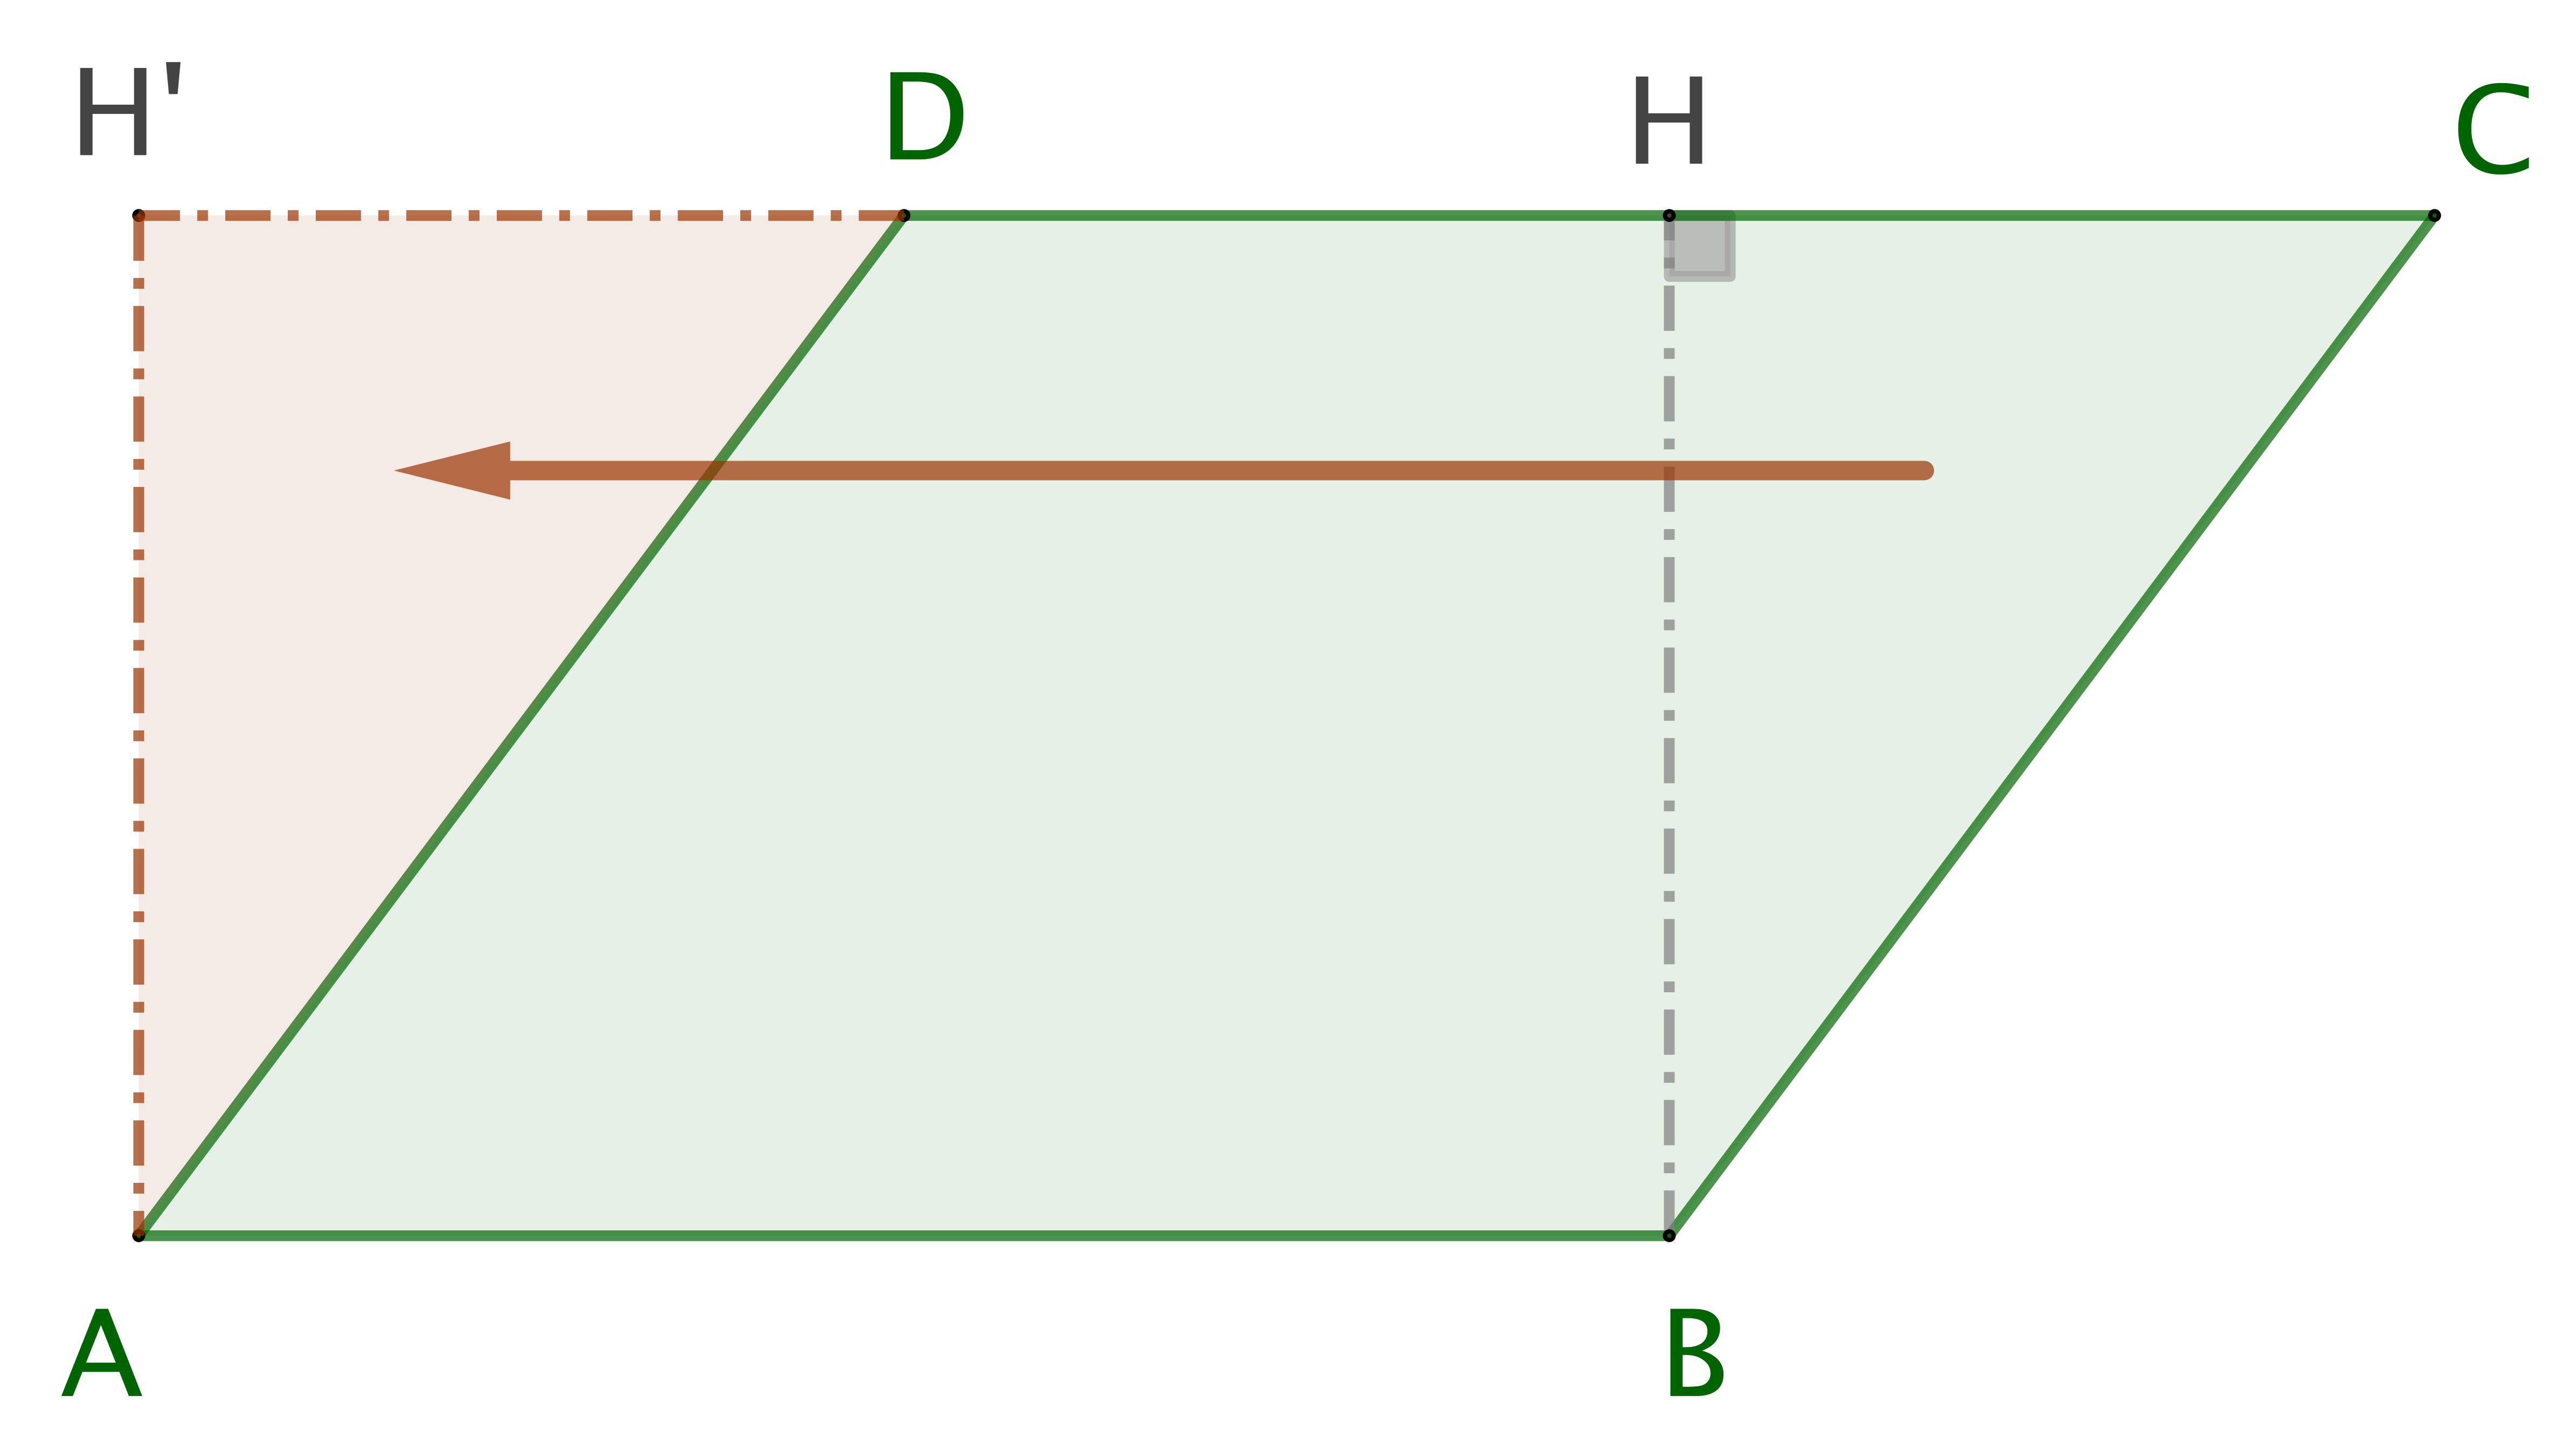
\includegraphics[scale=.4]{content/parallelogram/parallelogram.png}
	\end{center}
	
	Via une homothétie de rapport $k = \frac{\perim{ABCD}}{\perim{ABHH^{\,\prime}}} \geq 1$, nous obtenons un rectangle d'aire supérieure ou égale à $\area{ABCD}$, et de périmètre égal à $p$. Nous revenons à la situation du fait \ref{iso-rect} qui permet de conclure très facilement.
\end{proof}


\begin{remark}
	La recherche d'un parallélogramme de périmètre minimal pour une aire fixée est le problème dual de l'isopérimétrie pour les parallélogrammes.
\end{remark}


\begin{remark}
	Une méthode analytique devient pénible ici, car il faut par exemple prendre en compte l'angle au sommet $A$ du parallélogramme. L'auteur préfère battre en retraite en clôturant cette remarque ici.
\end{remark}
